\subsection{Soldado de Componentes}

Una vez que las placas fabricadas arribaron al laboratorio como en la figura \ref{placa_fisica} y todos los componentes de la plataforma se encontraban disponibles en el laboratorio, se comenzó el proceso de soldar el total de 180+ componentes discretos a la placa, que se completó en un marco de tiempo de aproximadamente tres semanas.\\

\begin{figure}[h]
    \centering
    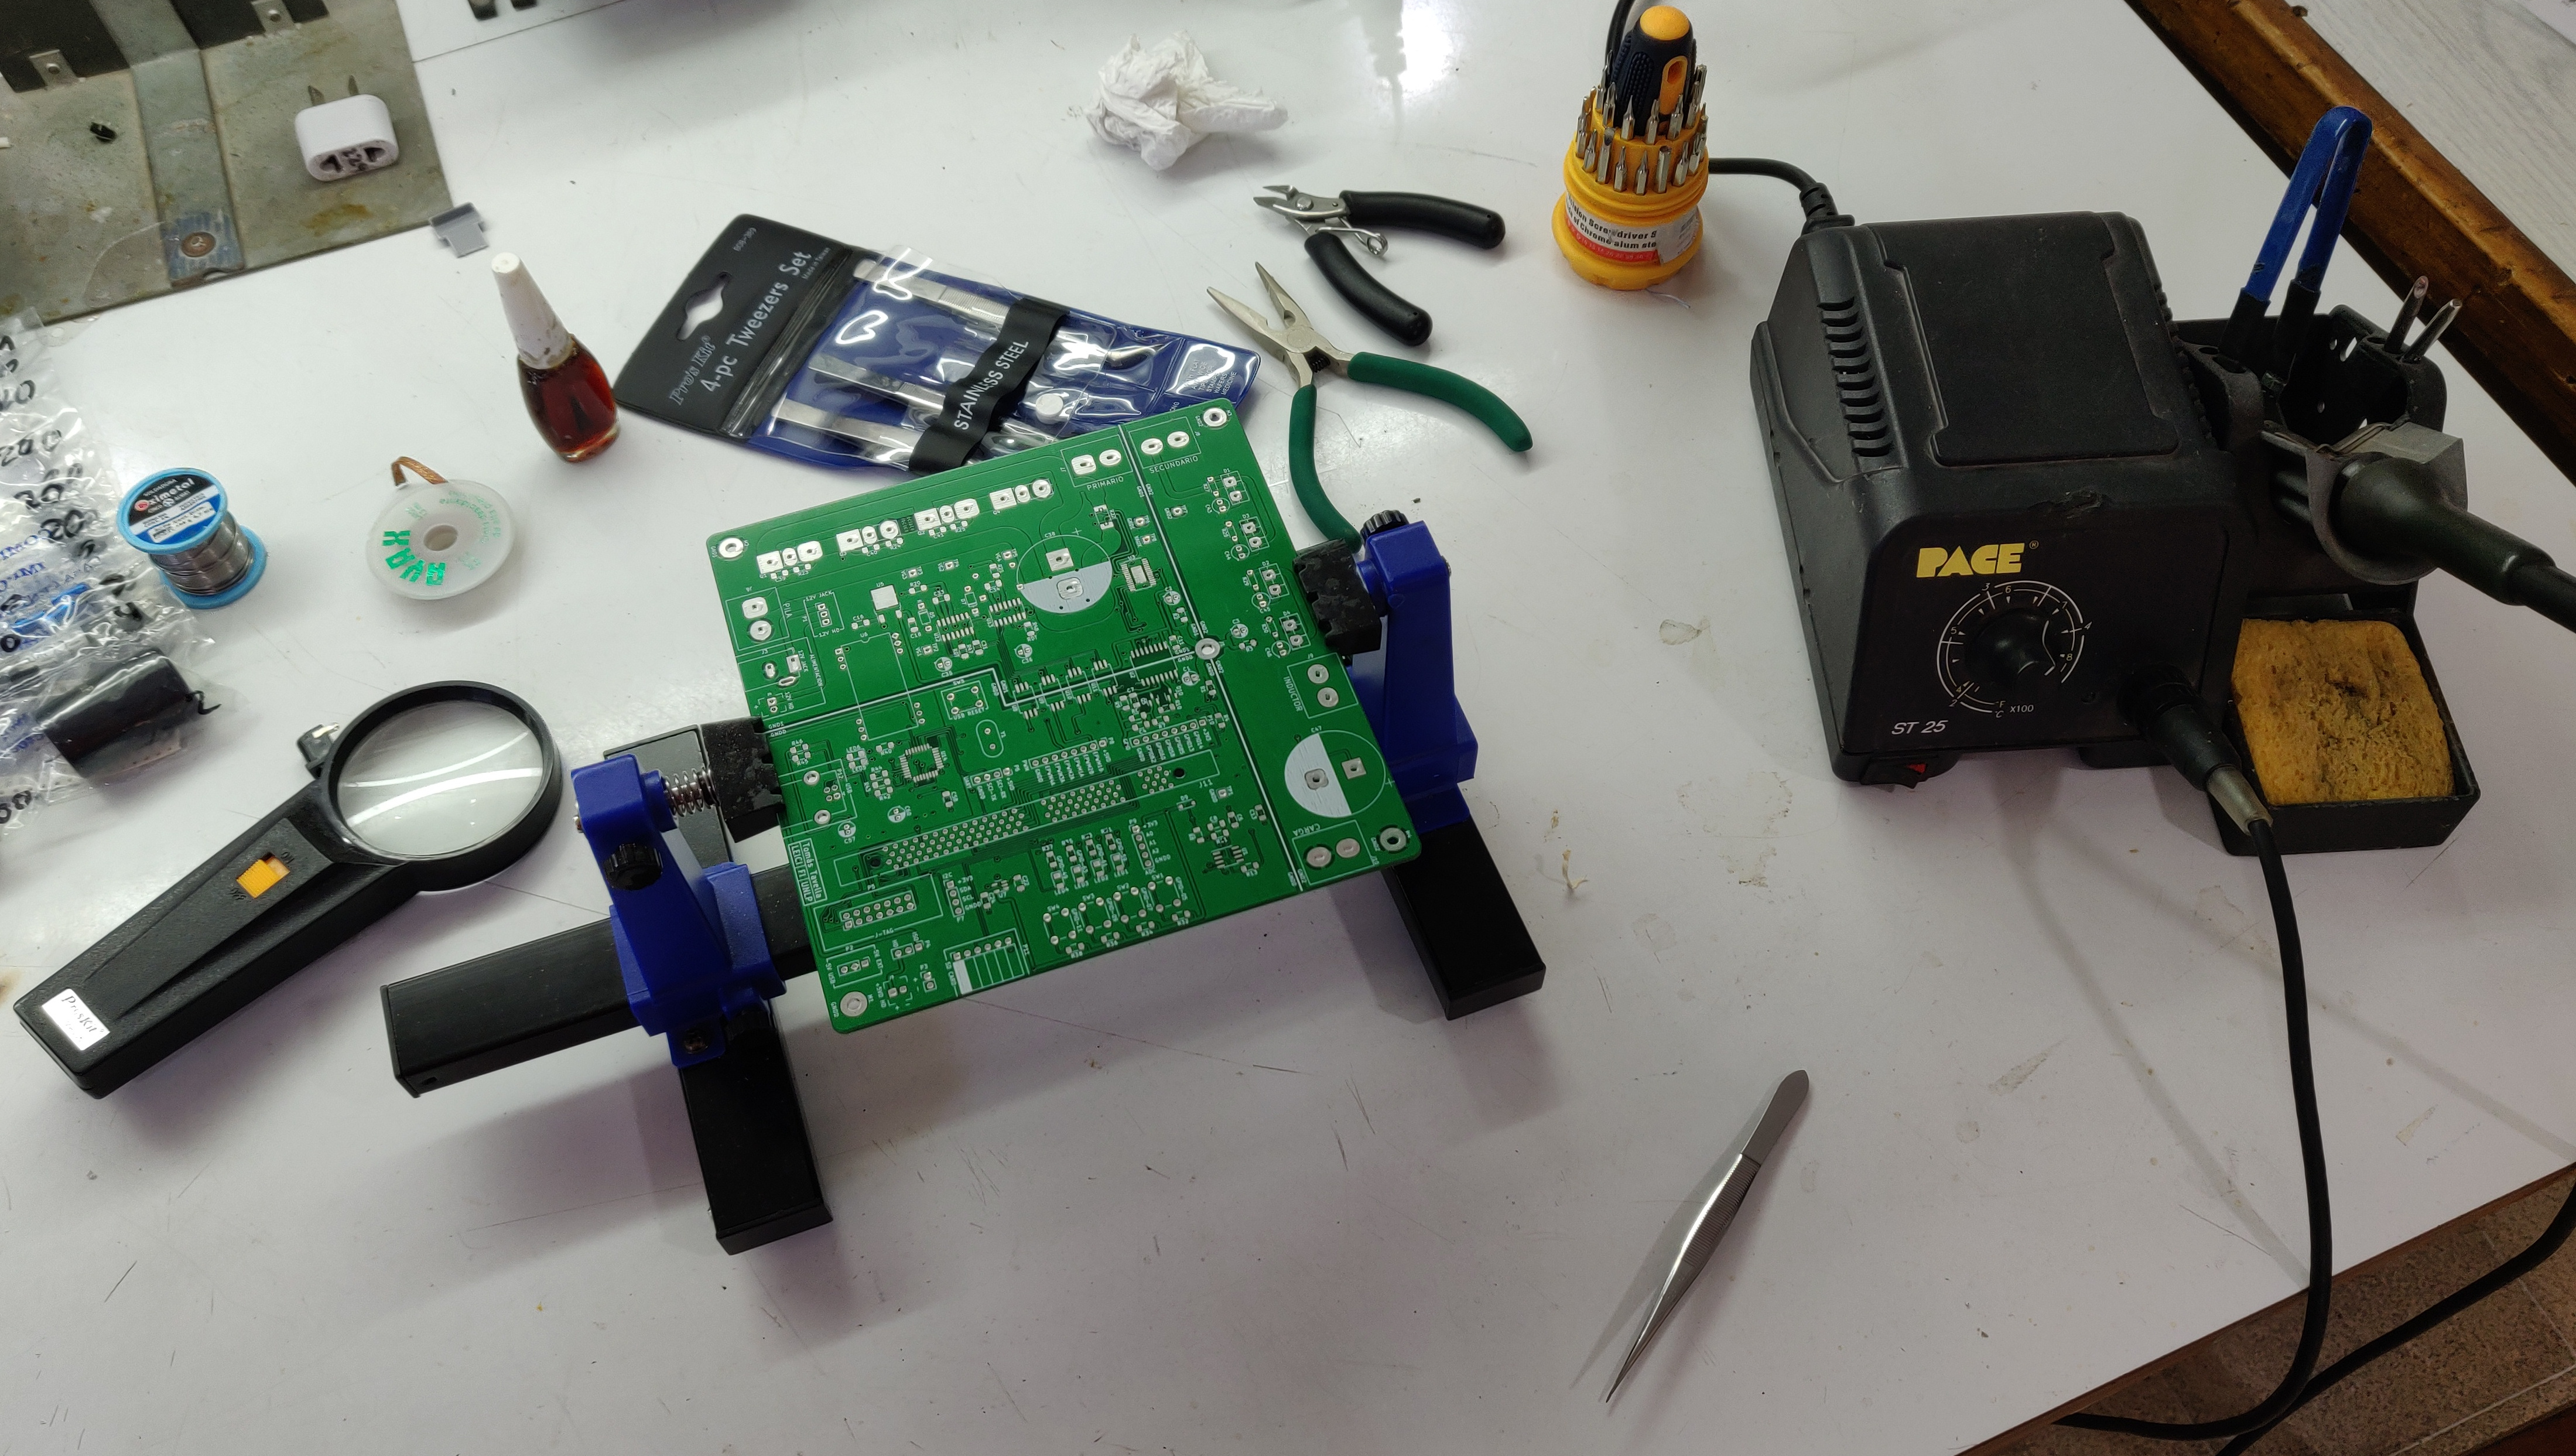
\includegraphics[scale=0.09]{Imagenes/Soldado.jpg}
    \caption{Zona de trabajo dónde se realizó el soldado de los componentes. A la derecha se puede observar la estación de soldado de temperatura regulable.}
    \label{soldado}
\end{figure}

Con asistencia del director del proyecto se aprendieron las nociones básicas de soldado de componentes SMD, y se completó todo el proceso sin mayores inconvenientes. Se comenzó soldando todos los componentes necesarios para evaluar el correcto funcionamiento del circuito driver y la excitación PWM, que incluyen los dos drivers medio puente de 2ED21834-S06J y todos su circuito auxiliar, los optoacopladores ACPL-P480 para aislar el DSC, el conector \textit{barrel} para la alimentación externa y el regulador lineal LM7805 para alimentar los optoacopladores.\\

Luego se continuó soldando el resto de los componentes, dejando los de mayores dimensiones físicas, en particular los capacitores de entrada y salida del convertidor, para el final del proceso, de manera que no estorben para la colocación de otros componentes.\\

El único componente que presento alguna dificultad al soldar fue el sensor LM5056A, cuyo empaquetado HTSSOP-28 cuenta con un pad encontrado en la parte inferior. En este caso, este pad es simplemente una conexión a tierra y cumple el único propósito de mejorar la capacidad de disipación térmica del dispositivo. Como no se cuenta con el equipo apropiado para soldar esta conexión, se utilizó una pasta térmica no conductora para al menos conseguir algín nivel de transferencia de calor del sensor al plano de tierra.\\